\documentclass[UTF8,a4paper]{article}% 文档格式
\usepackage{graphicx}
\usepackage{amsmath}
\usepackage{ctex}% 输出汉字
\usepackage{times}% 英文使用Times New Roman
\usepackage[left=1.50cm,right=1.50cm,top=1.80cm,bottom=1.50cm]{geometry}% 页边距设置
\usepackage{indentfirst}% 中文首行缩进
\renewcommand{\baselinestretch}{1.5}% 定义行间距(1.5)
\usepackage{fancyhdr} %设置全文页眉、页脚的格式
\usepackage{multirow} %Table Support
\usepackage{siunitx}
\usepackage{float}
\usepackage{ctex}
\title{\fontsize{14pt}{27pt}\selectfont% 四号黑体
    {\heiti% 黑体 
        基础物理实验报告\\
        光栅衍射实验}}
\author{\fontsize{12pt}{18pt}\selectfont% 小四楷体
    {\kaishu% 楷书
    杨哲涵~~~工物22班~~~2022011105}}
\date{2023年5月22日}
\begin{document}
\maketitle
\lhead{}% 页眉左边设为空
\chead{}% 页眉中间设为空
\rhead{}% 页眉右边设为空
\lfoot{}% 页脚左边设为空
\cfoot{\thepage}% 页脚中间显示页码
\rfoot{}% 页脚右边设为空
\section*{摘要}
\section{实验目的}
\begin{itemize}
    \item 进一步熟悉分光计的调整与使用。
    \item 学习利用衍射光栅测定光波波长及光栅常数的原理与方法。
    \item 加深理解光栅衍射公式及其成立条件。
\end{itemize}
\section{实验仪器}
\subsection{分光计}
分光计是实验用到的主要仪器,由平行光管、望远镜、度盘和平台构成。
度盘采用游标结构,由刻度盘(主度盘)和游标盘组成。该仪器有一旋转对称轴(主轴),刻度盘、游标盘平面垂直于主轴。度盘、望远镜、平行光管和平台等均可绕主轴旋转,
通过螺钉松、紧关系:可以实现某些部件的同步旋转(联动)、止动以及微动。

\begin{figure}[H] % 多图排版
    \centering
    \begin{minipage}[t]{0.5\linewidth}
        \centering
        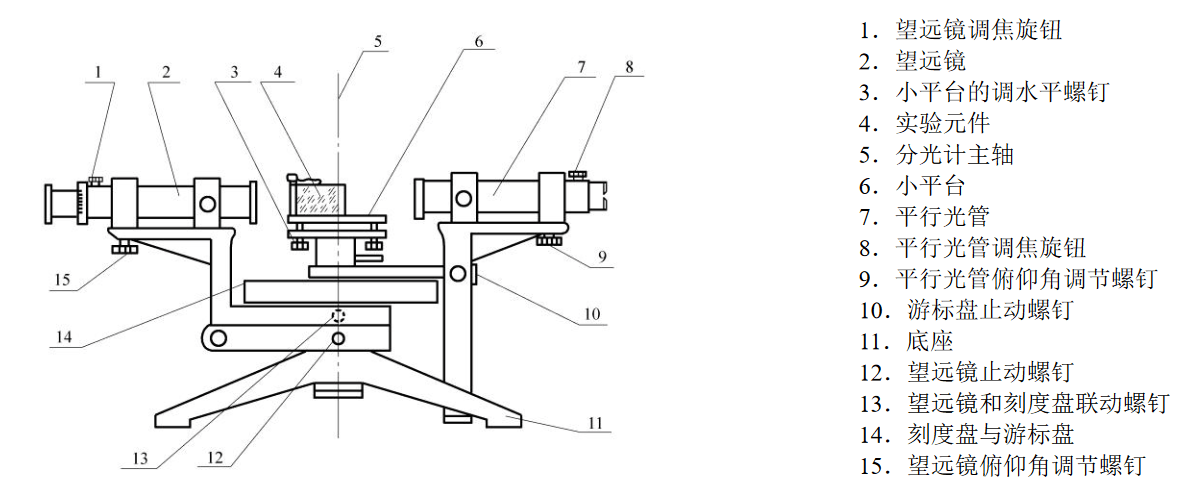
\includegraphics[width=0.95\linewidth]{分光计.png}
        \caption{分光计结构示意图}
        \label{}
    \end{minipage}%
    \begin{minipage}[t]{0.5\linewidth}
        \centering
        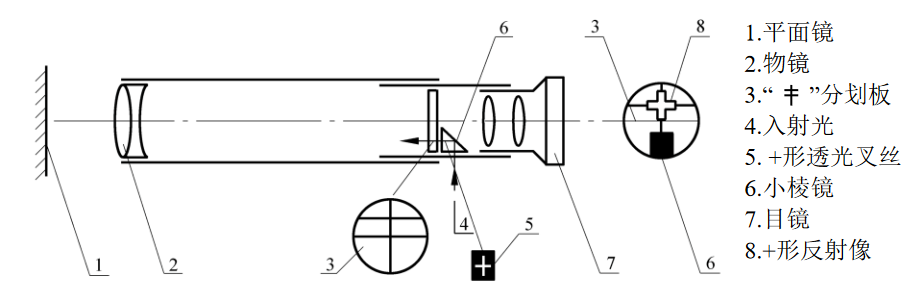
\includegraphics[width=0.95\linewidth]{望远镜.png}
        \caption{望远镜结构示意图}
        \label{}
    \end{minipage}
\end{figure}

\paragraph{望远镜}
实验用到的望远镜是自准直望远镜,由物镜、叉丝分划板和目镜组成,分别装在三个套筒上,彼此可以自由滑动。在调节望远镜时,应当使“干”形叉丝与“+”形透光叉丝的反射像均清晰成像。

\paragraph{平行光管}
平行光管由狭缝和透镜组成。狭缝与透镜之间距离可以通过伸缩狭缝套筒来调节。只要将狭缝调到透镜的焦平面上,则从狭缝发出的光经透镜后就成为平行光。

\begin{figure}[H] % 多图排版
    \centering
    \begin{minipage}[t]{0.5\linewidth}
        \centering
        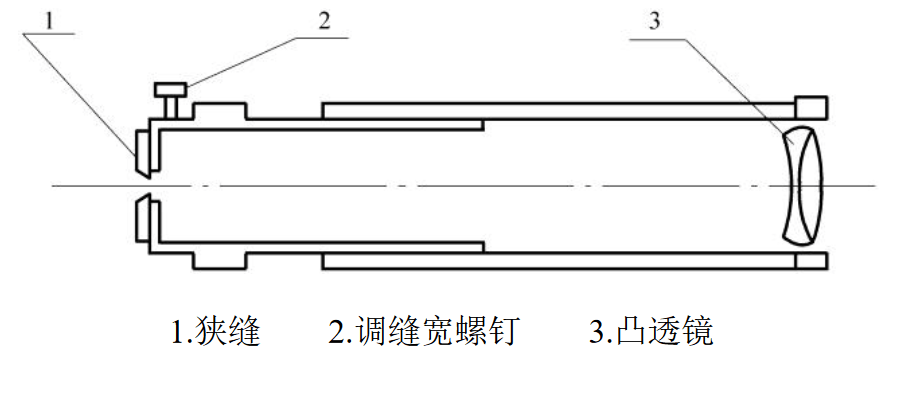
\includegraphics[width=0.95\linewidth]{平行光管.png}
        \caption{平行光管结构示意图}
        \label{}
    \end{minipage}%
    \begin{minipage}[t]{0.5\linewidth}
        \centering
        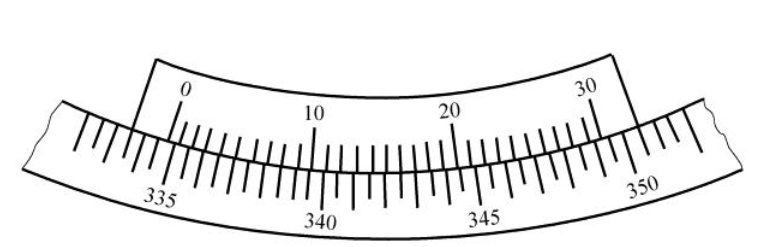
\includegraphics[width=0.95\linewidth]{刻度盘.png}
        \caption{刻度盘与游标}
        \label{}
    \end{minipage}
\end{figure}

\paragraph{刻度盘}
分光计的刻度盘垂直于分光计主轴并且可绕主轴转动。为消除刻度盘的偏心差,采用两个相差$180^\circ$的窗口读数。刻度盘的分度值为$0.5^\circ$,$0.5^\circ$以下则需用游标来读数。游标上的30格与刻度盘上的29格相等,故游标最小分度值为1分。
\subsection{光栅}
在本实验中应使光栅刻线与分光计主轴平行。如果光栅刻线不平行于分光计主轴,将会发现衍射光谱是倾斜的。通过调整小平台,可以使光栅刻痕平行于分光计主轴。
\subsection{汞灯}
本实验用到的汞灯在可见光范围内强度较高的谱线有四条,波长分别为$\qty{435.8}{nm}$(紫),$\qty{546.1}{nm}$(绿),$\qty{577.0}{nm}$(黄),$\qty{579.1}{nm}$(黄),它们也是本实验测量所用到的谱线。
在使用汞灯时,有以下注意事项:
\begin{enumerate}
    \item 汞灯在使用中必须与扼流圈串接,不能直接接 220 伏电源,否则要烧毁。
    \item 汞灯在使用过程中不要频繁启闭,否则会降低其寿命。
    \item 汞灯的紫外线很强,不可直视。如需观察,必须在狭缝前加一两层白纸以减弱其光强。
\end{enumerate}

\section{实验准备}
\subsection{实验原理}
本实验的基本原理为光栅衍射公式,设光栅常数为$d$,入射平行光与光栅法线成角度$i$,那么光栅衍射公式为:
$$d(\sin i\pm\sin\phi_m)=m\lambda$$
其中$\phi$为衍射光线与法线的夹角,两者分居法线异侧时取负号。$m=0,\pm1,\pm2,\cdots$其符号取决于光程差的符号。

特别地,正入射的情况下,$i=0$.

在本实验中,$i$已知,通过分光计可以方便地测出$\phi$,并且谱线的级别可以直接看出。若已知衍射光线波长$\lambda$,则可以得到光栅常数$d$,反之亦然。
\subsection{仪器调节}
\paragraph{定主轴}
这一过程需要调节小平台,使得分光计主轴在之后的测量中与光栅刻线平行。

为此可以使用手机的重力传感器,将手机(脱去手机壳为佳)放置在小平台上,调节小平台下的三个螺丝,直到手机重力传感器显示无任何偏移。
\paragraph{望远镜调节}
\begin{enumerate}
    \item 调节目镜,看清叉丝
    \item 将一反射镜贴在物镜镜头前,使得叉丝处发出的光被反射回目镜处,调节物镜直到能看清“+”字
    \item 将反射镜放在小平台上,旋转望远镜俯仰角调节螺钉,使得“+”字与叉丝上交点重合
    \item 取下反射镜
\end{enumerate}
\paragraph{平行光源调节}
\begin{enumerate}
    \item 将望远镜对准光源
    \item 调节平行光管伸缩套筒,直到狭缝线清晰成像
    \item 旋转狭缝,使得狭缝与“+”字竖线重合
    \item 调节狭缝宽度,保证像宽度$<\qty{0.5}{mm}$,以便减少长时间观察对眼睛的影响
    \item 调整平行光管俯仰,使得狭缝像在望远镜视场中间
\end{enumerate}
\paragraph{调光栅}
\begin{enumerate}
    \item 将反射镜放在小平台上,并且应调节至反射镜与望远镜方向垂直,在视场中相应位置能看到“+”
    \item 将光栅与反射镜平行放置,在视场中应当能看到两个“+”字像
    \item 调整光栅的放置角度,可以用指节顶在光栅边框从而小幅调节,使得视野中的两个“+”像的竖线重合
    \item 取下反射镜,保持光栅位置不动
\end{enumerate}
至此,仪器已经调整就绪,可以进行实验。
\section{实验任务}
\subsection{正入射}
在光线垂直入射光栅的情形($i=\ang{0}$)下,测定光栅常数与光波波长。
\paragraph{测定光栅常数}
实验准备时,已经使平行光垂直入射于光栅平面,因此可直接进行实验。

在实验中,记录1-5不同衍射级对应的绿光的衍射角$\phi_m$,约定汞灯绿线波长为$\lambda=\qty{546.1}{nm}$,可以得出对应$d$的值。

所得数据见表\ref{tab:lab1},我们选取第4级衍射级对应的数据进行计算,公式为:

$$U_{r}=\frac{U_{d}}{d}=\sqrt{(\frac{1}{\lambda}U_{\lambda})^{2}+(\frac{\cos\phi_{m}}{\sin\phi_{m}}U_{\phi_{m}})^{2}}$$
$$d=\frac{m\lambda}{\sin\phi_{m}}$$

注意波长为约定真值,因此$U_{\lambda}=0$,$U_{\phi_{m}}=\Delta_{\mathrm{INS}}$.带入数据得:

$d=\qty{3335.162175}{nm}, U_{r}=0.000335613$

最终测量结果为$d=(3335.2 \pm 1.1)\mathrm{nm}$.

\paragraph{测定黄线波长}
保持光栅位置不变,现观察汞灯长黄线,测量其衍射角并据此计算其波长。

在实验中共测得4组数据,使用第2级衍射级计算其波长,公式为:

$$\lambda=\frac{d\sin\phi_{m}}{m}$$
$$U_\lambda=\sqrt{\left(\frac{d}{m}\cos\theta\Delta_\mathrm{INS}\right)^2+\left(\frac{\sin\theta}{m}U_d\right)^2}$$

带入表\ref{tab:lab2}中数据计算得:

$\lambda=\qty{578.5433305}{nm}$,$U_\lambda=\qty{0.494652429}{nm}$

最终汞灯长黄线波长的测量结果为$\lambda=(578.54 \pm 0.49)\mathrm{nm}$.

对比汞灯长黄线波长约定真值$\lambda=\qty{579.1}{nm}$,测量结果涵盖该约定真值,结果有效。

\subsection{斜入射}
在$i=\ang{15}$时,测量汞灯光谱中波长较长($\qty{579.1}{nm}$)的黄线的波长。
\paragraph{调整夹角}
调整光栅平面法线与平行光管光轴的夹角为$\ang{15}$有多种方法:
\begin{enumerate}
    \item 利用已经测得的光栅常数$d$,按照斜入射公式计算对应汞灯绿线第2级衍射角$\phi_m$,将望远镜旋转到对应方位角后,旋转光栅,使得绿线第2级衍射谱线与视野中“+”像重合。此时完成了光栅平面的调整。
    \item 拧紧螺钉,使得小平台与游标盘一同旋转,旋转至游标盘上的刻度为$\ang{15}$,固定游标盘,此时完成了光栅平面的调整。
\end{enumerate}
\paragraph{测定黄光波长}
完成上述调整后,分别测量对应衍射级的衍射角,并判断衍射光线和入射光线位居光栅平面法线同侧还是异侧。
根据数据计算长黄线波长。

实验中所测得数据记录在表\ref{tab:lab3}中,按照斜入射计算公式可得:

\begin{table}[H]
    \centering
    \caption{斜入射黄线波长}
    \begin{tabular}{llllll}
        \hline
        衍射级别            & 1          & 2          & 3          & -1          & -2          \\
        衍射角             & \ang{4;58} & \ang{4;57} & \ang{15;1} & \ang{25;29} & \ang{36;50} \\
        是否同侧            & 否          & 是          & 是          & 否           & 否           \\
        波长$\mathrm{nm}$ & 574.45     & 575.49     & 575.78     & 571.75      & 568.10      \\ \hline
    \end{tabular}
\end{table}

注意这一测量结果与长黄线约定真值$\lambda=\qty{579.1}{nm}$相差较大,这是因为实验中调整$i=\ang{15}$不够精确,使得实际$i$有$\ang{;3}$左右的偏差。
\section{讨论}
\paragraph{仪器搭建}
在搭建仪器,校准光路的过程中,可以不拘泥于讲义上的方法,根据准确便利的原则,采用合适的方法调整光路。

例如,使用手机的重力传感器可以方便地大致保证小平台的水平放置,调节望远镜与光栅时均可使用反射镜,以便简化原先较为繁琐的操作。
\paragraph{测量偏差}
在测量光栅常数$d$的过程中,选择合适的衍射级别可以有效减少测量误差。

已知计算公式为:

$$\lambda=\frac{d\sin\phi_{m}}{m}$$
$$U_\lambda=\sqrt{\left(\frac{d}{m}\cos\theta\Delta_\mathrm{INS}\right)^2+\left(\frac{\sin\theta}{m}U_d\right)^2}$$

使用该公式对表\ref{tab:lab1}中1-5级绿线衍射角数据进行计算,可以得到:
\begin{table}[H]
    \centering
    \caption{正入射绿线衍射级对应不确定度}
    \begin{tabular}{llllll}
        \hline
        衍射级别                & 1        & 2        & 3        & 4        & 5        \\
        光栅常数($\mathrm{nm}$) & 3343.620 & 3337.836 & 3333.872 & 3335.162 & 3336.726 \\
        不确定度($\mathrm{nm}$) & 5.875    & 2.804    & 1.719    & 1.119    & 0.682    \\               \hline
    \end{tabular}
\end{table}
我们从中发现,衍射级别越高,误差越低,这是因为仪器误差限是固定的,在衍射角较大时,相对地,测量误差会更小。因此在实际数据处理时,选用了4级绿线衍射角数据进行计算。
\appendix
\section{原始数据}
注:征得实验指导老师同意后,原始数据采用电子表格记录,并未手写签字。
\begin{table}[H]
    \centering
    \caption{正入射绿线衍射角}
    \label{tab:lab1}
    \begin{tabular}{llllll}
        \hline
        衍射级别 & 1          & 2          & 3           & 4           & 5           \\
        衍射角  & \ang{9;24} & \ang{19;6} & \ang{29;26} & \ang{40;55} & \ang{54;55} \\ \hline
    \end{tabular}
\end{table}
\begin{table}[H]
    \centering
    \caption{正入射黄线衍射角}
    \label{tab:lab2}
    \begin{tabular}{lllll}
        \hline
        衍射级别 & 1          & 2           & 3           & 4           \\
        衍射角  & \ang{9;59} & \ang{20;18} & \ang{31;49} & \ang{44;00} \\ \hline
    \end{tabular}
\end{table}
\begin{table}[H]
    \centering
    \caption{斜入射黄线衍射角}
    \label{tab:lab3}
    \begin{tabular}{llllll}
        \hline
        衍射级别 & 1          & 2          & 3          & -1          & -2          \\
        衍射角  & \ang{4;58} & \ang{4;57} & \ang{15;1} & \ang{25;29} & \ang{36;50} \\
        是否同侧 & 否          & 是          & 是          & 否           & 否           \\\hline
    \end{tabular}
\end{table}

\end{document}
